\section{Introduction}
The Internet has fundamentally transformed the way humans interact. Over the next decade, the Internet of Things (IoT) will revolutionize manufacturing, energy, agriculture, transportation and other industrial segments of the economy which are estimated to be in the range of \$2.7 - \$6.2 trillion by 2025~\cite{manyika2013disruptive}. This significant development accompanies with the increase in equipment manufacturers, Internet service providers, and application developers. By the end of 2020, 212 billons IoT smart objects are expected to be deployed worldwide~\cite{gantz2012digital}. Machine-to-Machine (M2M)\index{M2M} traffic flows will constitute up to 45\% of the whole internet traffic in 2022~\cite{taylor2013next},~\cite{evans2011internet}. Additionally, the Industrial Internet (IIoT, Industry 4.0)\index{IIoT} is predicted to create about 1279 billion dollar in 2020 according to Wikibon report~\cite{floyer2013defining}.\\

While Industrial IoT offers infinite potentials and opportunities for current industries and their process transformation, achieving interoperability is still a major challenge due to lack of uniform standards. One of the emerging technologies to overcome this challenge is IoT middleware. It is a software system implemented as a middle layer between device and application layers. The IoT middleware provides a set of programming abstraction to cover the heterogeneous things and low-level communication between IoT devices and end-user applications~\cite{fersi2015middleware}. Global Sensor Network (GSN)\index{GSN}, Xively, Paraimpu, ThingWorx are some of the major middleware solutions used in similar context. These systems share a common objective of achieving seamless integration of heterogeneous things into the Internet with different approaches. For example, GSN uses a concept named wrapper to handle the connection from sensor hardware to middleware. Hydra, ThingWorx offer a Device Development Kit to create the applications on device side. However, these approaches require programming skill and a lot of effort to establish and configure connectivity for new IoT object, which do not appropriate for non-specialist users. In case of GSN, in order to establish the connection from sensors to middleware, we must build an executable file named wrapper and a corresponding configuration file for every sensor using provided library. \\

Due to heterogeneity in IoT environment, each IoT object such as sensor and actuator provides different software interfaces and communicating configuration to exchange data and control information with cloud-base middleware. Furthermore, these interfaces and configuration are non-standardized and frequently changing, expecially in a Low Power Wide Area Network (LPWAN) senario. Moreover, to retrieve the monitoring data from IoT devices using LoRa  connection, we have to configure an HTTP callback following special format which is defined by a network provider. However, each provider has various configuration formats and frequently changes that lead to a giant gap in syntactical interoperability and stability.\\

In the IoT era, data processing plays a tremendous role in analysis, prediction and context-awareness. Along with the exponential growth of the open data services (ODS), interoperating between these services and IoT middleware is challenged by heterogeneity. Most of the ODS follow a client-server model built using RESTful web service. However, each service provider offers a diverse HTTP configuration (path, method, header), data format (JSON, XML) and data syntax. For examle: ``Accuweather'', a weather data sharing service, configures identification key as a parameter in the URL namely ``apikey''. However, ``Openweather'' service configures identification key in the HTTP header. Therefore, a new mechanism to deal with heterogeneity syntax of IIoT connectivity should be considered.\\

In this chapter, we present a novel Industrial IoT framework to support automatic establishment and configuration process for heterogeneous connectivity by using a system-generated connector. The connector is a specific code segment that performs the data acquisition process from a specific type of connection using protocols like HTTP, MQTT. Our framework also provides APIs to perform full ``create, read, update, delete'', CRUD operation on the connectors. Furthermore, automating connectivity mechanism assists end-user in quickly retrieving data from various data sources via self-defined connectors. These connectors also allow explicitly specifying the information to be collected. For example, we can create a connector to retreive only current temperature and humility amongs deverse data of open weather data sources. Thus, this mechanism enables the middleware to accelerate data acquisition process. Especially, our proposed framework is extremely fit for LPWAN scenario which lacks of uniform data and interoperation between network provider. Moreover, sensing data of LPWAN devices is restricted due to low data rate and bandwidth. Thus, enriching data from open data sources is extremely necessary for this scenario to gain maximum benefit from data analysis and context-awareness. To demonstrate the capability of this framework, we integrated it into an existing middleware to evaluate the performance. \\

The main our contributions are:
\begin{enumerate}
    \item Identifying current middleware limitations for connectivity and automatic configuration for IIoT.
    \item Proposing a novel and lightweight framework to accelerate the connecting process for heterogeneous things.
    \item Utilizing the proposed framework to speed up the data acquisition from open data sharing web services.
    \item Simplifying connectivity management by wrapping connectivity object in a RESTful web service.
    \item Implementing and evaluating the proposed framework.
\end{enumerate}

\section{Related Work}
In this section, we review the connectivity mechanism for IoT device in some current frameworks. We also identify their limitations to motivate to deliver a novel IIoT framework that simplifies the establishing and configuring connectivity to IoT things using the system-generated connector.

\begin{description}
    \item [FIWARE] is cloud-based middleware platform that provides an infrastructure to effectively reduce the cost of creation and delivery IoT services by sharing and re-using Generic Enablers (GE)~\cite{zahariadis2014fiware}. All API and GE specifications are public and royalty-free for all developer. These documents contain the necessary information to create an IoT product that can interoperate with other developed GE in FIWARE community. The other innovative aspect of FIWARE is that all IoT things are covered behind OMA Next Generation Service Interface (NGSI) entities. Therefore, developers just need to learn and work with the NGSI API used in FIWARE regardless the complexity of IoT technologies and deployment. To handle messages from the IoT devices and gateway, FIWARE provides an element namely IoT Agent. The main responsibility of this element is receiving and translating the messages to a uniform format. Currently, FIWARE IoT Agent supports HTTP and MQTT~\cite{iota-fiware-iot-stack}. However, creating a new IoT Agent involves a lot of effort to understand the FIWARE framework  which is only used by developer. Regarding integration with data sharing service, FIWARE proposes Cygnus, a connector between Orion Context Broker to certain FIWARE storage such as CKAN, HADOOP, DynamoDB. Cygnus is based on Apache Flume  which supports collecting data via persistence agents. Basically, Cygnus only supports some specific HTTP Flume agents. That means, FIWARE is able to integrate with a few supported data sources.
    
    \item [Global Sensor Network] is a platform aimed to provide a flexible integration with different type of sensors. GSN facilitates the connecting process of heterogeneous sensor devices to an application by implementing a corresponding wrapper and an XML file~\cite{Aberer2006}. This XML file defines the basic configuration information for the sensor such as the type of data will be sent to GSN, parameters, and the corresponding wrapper. The wrapper acts as a sensor driver to establish a connection from sensor hardware to GSN. These two elements must be created for every sensor which demands to connect to GSN. Currently, creating the wrapper and establishing the connectivity are complicated tasks and require high programming skill~\cite{gsn_2013}. Another critical drawback of GSN is that all sensor data is stored in an SQL database. This leads to a limitation in performance and scalability.
    
    \item [Hydra] Hydra middleware project aims to develop a service-oriented middleware for physical devices in a distributed architecture, also known as Link Smart~\cite{eisenhauer2009development}. This framework is developed based on Service Oriented Architecture (SoA), which uses web services for seamless integration of heterogeneous physical devices into applications regardless connectivity technologies. Hydra also provides a dedicated access control mechanism to ensure the authorization and privacy for all IoT services and devices. The Hydra IoT devices are described by using semantic technologies. Thus, the new devices can be discovered automatically in the Hydra Network using peer-to-peer network technology. Hydra also provides the set of development resource to create an application on both device and end-user side including the Software Development Kit (SDK) and the Device Development Kit (DDK). But, both SDK and DDK are complicated to be used by end-user. In addition, creating a new device template or Hydra IoT Application must be implemented by a programmer. Therefore, this middleware is not suitable for the end user to quickly create or deploy the IoT devices, services or applications. The other limitation of Hydra is that the Hydra device application interacts with middleware using web service. Thus, this application is too heavy to run on constraint IoT devices which limit to memory size and processor.
    
    \item [Kaa] Kaa project is open-source IoT middleware platform with a lot of IoT features that allow the users build the complete end-to-end IoT solution including data management, data connection and configuration management~\cite{kaa_project}. Kaa middleware uses data scheme and configuration scheme to configure IoT devices in term of data structure and device configuration. These schemes are created and managed by Common Type Library (CTL). It also provides a SDK to create the embedded application for IoT device in several programming languages such as C, C++, java and Objective C. However, the limitation of Kaa middleware is that the endpoint SDK only supports few specific IoT devices and the interoperation with other data sources is not mentioned.
    
    \item [Xively] is a cloud-based platform using a central message bus to route the message from devices to another platform components. This platform provides many development tools and resources supporting developer connect and obtain data from their sensors. The IoT sensors can connect to Xively via MQTT, HTTP and Web Socket protocol~\cite{kohler2014platforms}. However, the principal purpose of Xively is just to simplify the connecting from the sensors to Xively’s Cloud. Therefore, in case we need an additional service, we need to develop a new one or reuse compatible service with Xively. Adding a new sensor to Xively is supported to be uncomplicated, but the provided API is hard to use, especially for the unsupported sensor. Furthermore, there is no the function using to integrate with open data sources via web service. These limitations lead to the restricted usage for inexpert users.
    
    \item [ThingWorx] ThingWorx platform addresses IoT application integration that monitors, manages and controls connected devices through model driven development. All sensors, applications, and services are treated as data sources and inter-connected via virtual bus~\cite{derhamy2015survey}. The platform supports several connection protocols including CoAP, MQTT, REST/HTTP and Web Socket. It also supports integrating with other sharing data sources via web services including open weather services, social data providers. However, ThingWorx only supports a few web services, and not allow the user to establish the integration to new web service. The other limitation of ThingWorx is that devices only allow connecting to ThingWorx’s Cloud by using the applications to be implemented by ThingWorx SDK~\cite{solutions25platform}.
    
\end{description}

\section{Problem Statement}
 Most of the studied platforms limit the type of sensor that can be connected and request a specific application installed on device side. Also, adding a new sensor to the platforms is complex and require advanced programming skills. There is no mechanism to deal with the rapid changes things in term of software interface, connectivity protocol and data format. Moreover, reviewed frameworks do not support the end-user to establish connection and collect data from open data sources via HTTP, MQTT, CoAP or WS protocol. Our framework has been designed and developed to overcome with these limitations.
 
 
\section{IoT Framework for Connectors}
This section concentrates on our middleware architecture, connector management mechanism and connector generation process along with its elements. At the end of the section, we describe different deployment scenarios to emphasize its high compatibility with various parts of IoT system.

\subsection{System Architecture Overview}

\begin{figure}[h!] 
 \begin{center} 
 \includegraphics[width=0.72\textwidth]{./Part2/Chapter4/figures/connector_architecture.png} 
    \caption{The overview of framework architecture.}
     \label{fig:c4_overview_architecture}
  \end{center} 
\end{figure}

Our framework simplifies the creation and management process for heterogeneous connectivity. Our approach is to wrap the complex establishing and connecting functionalities in the RESTful web services which are easily handled by end-user. Fig.~\ref{fig:c4_overview_architecture} depicts the proposed framework which is composed of three different layers described below.
\begin{itemize}
    \item \textbf{Service Enablement Layer:} This layer consists of several web services which allow the end-user a direct interaction with the framework. The supported operations are (i) discovering connector, (ii) CRUD operations on connector and connector template, (iii) activating, de-activating connector and (iv) access control based on session token. There are four main services are connector management, connector discovery, access control and connector template management. These services allow the end user to establish and manage connectivity to IoT devices as well as various data source simply regardless the complexity of protocol and configuration process through RESTful web service. This capability is essential and important for adapting to the lack of standardization and the rapid changes of IoT thing. However, it is not supported by the reviewed IoT platforms.
    \item \textbf{Processing and Storage Layer:} This layer contains the databases and primary functions to generate the connectors as well as pre-process data. It also carries a database to store generated connector, connector template, and connector status. The connector creation process is performed and managed by connector generation service. This service generates the connector from connector template which is configured and sent by the end user via connector management service.
    \item \textbf{Connection Layer: } This is composed of many generated connectors that have the responsibility to handle the connection to IoT things. Currently, our framework supports two types of connectors - ‘Connector In’ and ‘Connector Out’. They are analogous to ‘proxy-in’ and ‘proxy-out’ concepts introduced in~\cite{datta2014iot}. Each type of connector supports HTTP, MQTT, CoAP and WebSocket (WS) connectivity respectively to retrieve data from sensor, actuator, gateway and open data sharing services. This is extending the ``collection proxies'' concept presented in~\cite{datta2016easing}. This layer also keeps tracking the connector status via connector management module. The end user can manage this status by calling the appropriate web service. 
\end{itemize}
\subsection{Connector Generation Elements}
To facilitate the connectivity generation for end-user, we propose the Connectivity Configuration Template (CTT) file, contains the vital information of seeking connectivity such as connection properties, data description. This file is encoded under XML format which provides simplicity, openness, and extensibility. The CTT’s content is coherent and convenient for both human and machine. Moreover, the structure of CTT is roughly equivalent to a network packet corresponding to the supported connection. Fig.~\ref{fig:c4_connector_operation} illustrates an example of complete CTT file to establish an HTTP connection to acquire the data from Accuweather, an open data sharing service about weather information.\\

\begin{figure}[h!] 
 \begin{center} 
 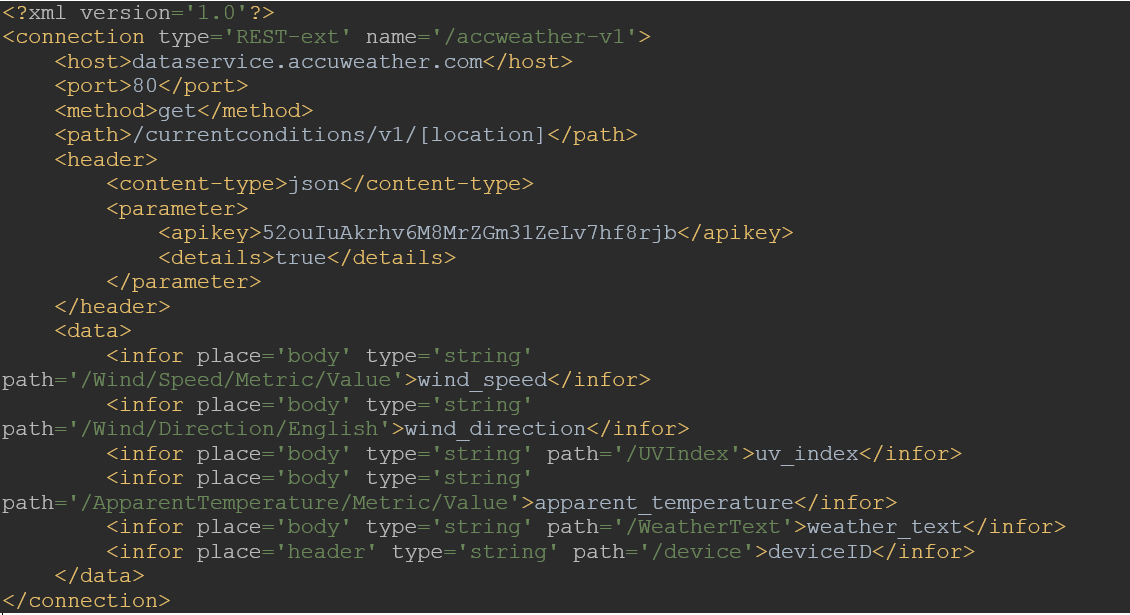
\includegraphics[width=0.72\textwidth]{./Part2/Chapter4/figures/connector_template.png} 
    \caption{An example of Connection Template.}
     \label{fig:c4_connector_template}
  \end{center} 
\end{figure}

From Fig.~\ref{fig:c4_connector_template}, the necessary connection properties are a host address, port number, connection method, path address. The header element defines the operating information of HTTP transaction such as content type, authentication information and HTTP parameters. The next element describes the carrying payload in the HTTP packet. Each data in the payload is defined by one ``infor'' tag that has three attributes including (i) ``place'' which describes the HTPP object storing the payload such as HTTP body or HTTP header, (ii) ``type'' which describes the type of the data such as string or number, (iii) ``path'' which defines a specific location of data in the payload.\\

The connector is a piece of JavaScript code, which has a responsibility to open connectivity and perform data acquisition. It is also able to annotate the raw data by using define vocabulary which increases the interoperability. The connector structure consists of three distinct parts with the different responsibility to (i) open the connection based on the received in the CTT file, (ii) de-capsulate and process the data from the received network packet and (iii) manage the connector status via web service. The connector functionalities are not only triggered by incoming network packet but also by defined interval time to obtain data from open data sharing services. In order to facilitate the management process, the framework uses a brief and a unique name to identify connector. In case multiple devices connect to the same connector, these devices are identified by their ID. The position of device ID is configurable in connector. For example, in Fig, 2, device ID will be retrieve via ``device'' parameter in HTTP header. The connector is created by combining CTT and Connector Template (CT). CT is a composed script with the marked position which is filled by the extracted information from CTT to create the connector. Each type of connector has different CT.

\subsection{The Framework Process}

The primary task of our framework is presented in Fig.~\ref{fig:c4_connector_general_operation}. In order to create and effectively manage the connector, the end-user must follow these steps. Firstly, they send the connectivity protocol used (e.g., HTTP, MQTT) to the framework via RESTful web service and then the framework response a CTT file corresponding with their demand. Secondly, the end-user fills received CTT file with connectivity configuration information such as host address, port number and send this CTT file to framework to trigger the connector generation process. Finally, the framework automatically generates the connector base on CTT file from user and response generating status along with connector name to the user. After generating, this connector is available to receive or obtain data from IoT things as well as be managed via web services.

\begin{figure}[h!] 
 \begin{center} 
 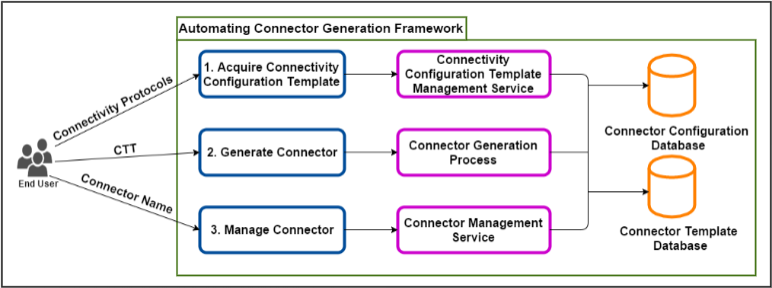
\includegraphics[width=0.72\textwidth]{./Part2/Chapter4/figures/connector_general_opereration.png} 
    \caption{The framework in operation}
     \label{fig:c4_connector_general_operation}
  \end{center} 
\end{figure}


\subsection{Connector Generation Process}
The connector generation is triggered when receiving a creating connectivity requisition from end-user via Service Enablement Layer. This request carries the CTT file which contains the necessary configuration to establish connection encoding under XML format. CCT can be delivered to end-users in advance by RESTful web service to supports the non-specialist end-user in creating connectivity. The framework extracts the vital information in received CTT and assigned this information to an array following a certain order. The next operation is to inject these values into the correct positions in CTT file. After successfully creating, the new connector is stored in database and register with connection layer to be available. The overall process is illustrated in Fig.~\ref{fig:c4_connector_operation}.

\begin{figure}[h!] 
 \begin{center} 
 \includegraphics[width=0.72\textwidth]{./Part2/Chapter4/figures/connector_operation.png} 
    \caption{The operational diagram.}
     \label{fig:c4_connector_operation}
  \end{center} 
\end{figure}

\subsection{Connector Management}
In order to control the connectors from end-user, we propose Connector Management Component (CMP) which is located in Connection Layer. CMP manages all existing connectors following Resource Oriented Model.  Each connector is identified via unique connector name which allows connector resources to be discovered by ``Connector discovery'' component in Service Enablement Layer. \\

At first declaration, the framework will automatically register the new connector with CMP by its name. After successful registration, CMP will allocate a set of RESTful web services to registered connector. Our framework supports basic management actions on a connector including CRUD, activation and deactivation. For instance, after successful creating, a connector is associated with ``active'' status and ready for operating. The end-user can deactivate the connector by triggering ``deactivate'' action.
\subsection{Deployment Scenarios}
Our framework is implemented using Node.js programming language, a JavaScript runtime built on Chrome's V8 JavaScript engine using an event-driven, non-blocking I/O model~\cite{joyentnodejs}. Therefore, it is extremely lightweight to be efficiently deployed in the wide range of the M2M objects such as a gateway, cloud-based system and even smartphone. This capability makes the framework are flexible to integrate into various parts of IoT ecosystem. For a large-scale enterprise using various technologies to communicate, our framework can be deployed to the gateway to facilitate the connection process for new devices and easily adapt to the changes of configuration from network providers and new coming connectivity standard. In the real scenario, the framework is deployed in a cloud-based system using to simplify connectivity to devices via LPWAN connectivity. In the other perspective, our framework can be implemented as a data acquisition layer in other frameworks such as SIGHTED~\cite{nagib2016sighted} or as a proxy layer in a lightweight Framework for efficient M2M device management in oneM2M Architecture~\cite{datta2015lightweight} to accelerate the connection process.


\section{Evaluation}

To evaluate our framework, we propose to measure the execution time of connector generation process including two main operations, namely connector creation and reloading framework

\begin{itemize}
    \item \textbf{Connector creation operation: } The operation performs the combination of CTT uploading from end-user and CT storing in the database to generate the target connector.
    \item \textbf{Reloading framework operation: } After the finish of connector generation process, this operation occurs to integrate new connector into the framework.
\end{itemize}

We recorded the execution time in seconds of 50 times wrapper generation process with the wrapper configuration is 852 bytes. The evaluation is performed on-device has the processor: Intel(R) Core(TM) i5-6200U CPU @ 2.30 GHz, 2401 MHz, 2 Core(s), 4 Logical Processor(s), 4 GB of RAM and the operating system is 64-bit Windows 10. The acquired result is shown in Figure 6. According to that, reloading framework takes around 1.15 s to 2.91 s while the connector creation operation only consumes around 0.113 s to 1.4 s. Overall, the total execution time is from 1.265 s to 4.31 s. This performance satisfies the user experiment~\cite{rosson2002usability}. When the connector works as a ``proxy out'', the time of establishing connection is extremely minor around 0.003 ms comparing with the total time which is largely depended on the performance of the data sources. In addition, most of open data sources are limited in the performance and the number of request could be served per second. \\

\begin{figure}[h!] 
 \begin{center} 
 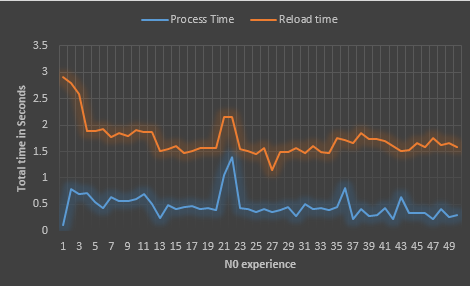
\includegraphics[width=0.72\textwidth]{./Part2/Chapter4/figures/connector_performance.png} 
    \caption{Connector generation performance}
     \label{fig:c4_connector_performance}
  \end{center} 
\end{figure}

The size of connector for each M2M connectivity is less than 1 KB, and the requested memory of our framework is only a couple of megabytes of memory. Thus, our framework is satisfactory to deploy on the general IoT objects from cloud-base middleware, M2M gateway and event smartphone with gigabytes of internal memory along with the powerful processor. It further demonstrates the ultra-lightweight of the proposed framework. In the other hand, the size of CTT only depends on the data section. However, this section is not processed or participated in connector generation process. Therefore, the performance of connector generation process is independent of the size of CTT. Furthermore, the connectors are developed Node JS Express framework  supporting non-blocking I/O model, and consequently, there is unlimited in the number of devices connecting to a connector. These properties make the framework more scalable and flexible to be deployed in the large-scale scenario.

\section{Conclusion}
In this chapter, we identify the limitations of some existing middleware solutions regarding the data acquisition and configuration connectivity. Motivating to bridge the gaps, we proposed a framework that can simplify the establishing connection process from IoT things to cloud-based middleware via a system-generated connector. Our platform also provides well-supplied management web services based on resource oriented model. It allows the end users to easily discovery and perform a wide range of management operation on the connector including creating, retrieving, updating and deleting as well as activating or de-activating. Another innovative aspect is that the connector can facilitate and speed up the data acquisition process from data sharing web services such as Accuweather, OpenSensorIO. In evaluation section, we demonstrate the scalability and flexibility of our platform via satisfactory performance, lightweight software implementation and low memory consuming. Regarding future works, we are working on integrating our platform into oneM2M architecture and implementing access control mechanism.

